\section{Fluctuation dissapation theory from Brian Cowans Notes}
\label{sec:fluctuationDissapation}

\subsection{Summary}
\begin{itemize}
\item How correlation functions of voltage  and current can be integrated to give
  the resistances in a given circuit:
  \[
    {R}                                                                         =
    \frac{1}{2kT}\int\iaverage{V(0)V(t)}dt\qquad\frac{1}{R}=\frac{1}{2kT}\int\iaverage{I(0)I(t)}dt.
  \]
\item When a system feels an effect $ B(\tau) $, it responds with $ M(t) $ according
  to the dynamical susceptibility $ X $.

  \begin{framed}\noindent
    \begin{equation}
      M(t) = \int_{-\infty}^{t}X(t - \tau)B(\tau)d\tau.
    \end{equation}
  \end{framed}
\item For a sinusidal excitation $ B(t) = be^{-i\omega t} $ the response is
  \begin{framed}\noindent
    \begin{equation}
      \begin{aligned}.M(t)    &=    be^{-i\omega   t}\chi(\omega)\\    \chi(\omega)    &=
        \int_{-\infty}^{\infty}X(\tau)e^{i\omega t}dt
      \end{aligned}
    \end{equation}
  \end{framed}

  The  real and  imaginary parts  of dynamical  susceptibility are  even and  add
  respectively.

\item Working in frequency domain
  \begin{framed}\noindent
    Given a superposition of forces (expressed  by $ b(\omega) $ in the frequency
    range)
    \begin{equation}
      B(t)     =    \frac{1}{2\pi}\int_{-\infty}^{\infty}b(\omega)e^{-i\omega
        t}d\omega,
    \end{equation}
    \noindent the response can be found by evaluating the response at frequency:
    \begin{equation}
      m(\omega) = \chi(\omega)b(\omega),
    \end{equation}
    \noindent and  `summing' them up, which  is equivalent to taking  the fourier
    transform
    \begin{equation}
      M(t)     =    \frac{1}{2\pi}\int_{-\infty}^{\infty}m(\omega)e^{-i\omega
        t}d\omega.
    \end{equation}
  \end{framed}
\end{itemize}


  \subsection{Correltion function}
  The correlation function
  \begin{equation}\label{eqn:corr1}
    g(\tau) = \iaverage{X(0)X(\tau)} - \iaverage{X^2},
  \end{equation}

  \noindent measures how  fast variations in a system will  go away.  Effectively
  what is happening is  we are averaging the fluctuation $ X(t)  $ over time from
  its equilibrium value $ \iaverage{X} $.  Of course, a decay should slowly decay
  (on  average,   and  hence  that   is  why   we  take  the   expectation  value
  $ \iaverage{X(t)} $).

\begin{figure}[h]
  \centering 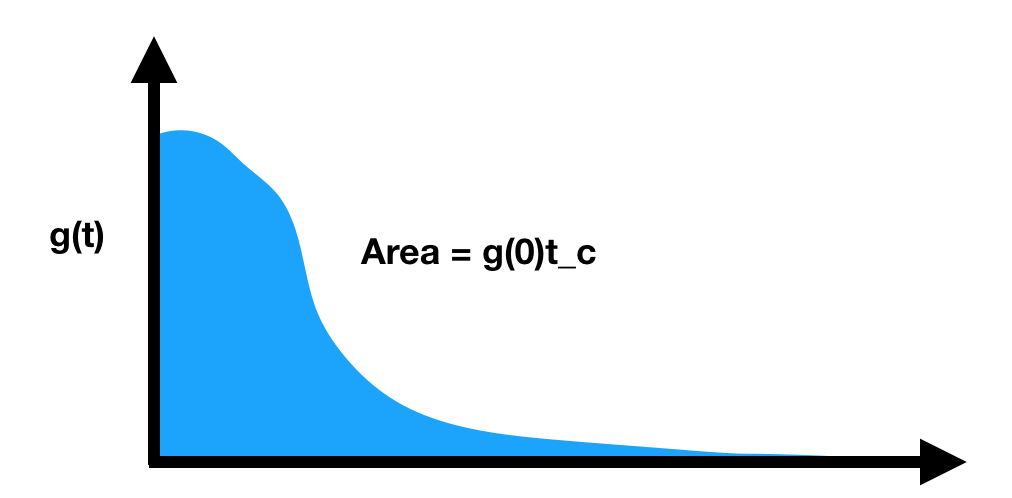
\includegraphics[height=5cm]{g1_decay}
\end{figure}

\red{Because fluctuations are symmetrical about the equilibrium value, we need to
  multiiply the fluctuation by its initial value  $ X(0) $ to avoid averaging out
  to 0.  \textit{This is a very clever trick indeed.}}

 \subsection{Fluctuation dissapation theory}\label{subsec:fluctuationDissapation}
 This  is  a   very  general  theory,  applied  here  for   current  and  voltage
 respectively. The idea is to write out  the dynamics of one variable, and equate
 the energy found to  the energy available.  This contrains the  value of some of
 the parameters.

 \begin{enumerate}
 \item Write out the equation of motion:
   \begin{equation}\label{eqn:corr_2}
     L\frac{dI}{dt} + RI(t) = V(t) \quad (\text{Kirchoffs 2nd})\qquad\qquad C\frac{dV}{dt} + \frac{1}{R}V(t) = I(t) \quad \text{(Kirchoffs 1st)}.
   \end{equation}
 \item Propose  a trial solution (this  is called the integrating  factor method,
   and I covered on Wikipedia):
   \begin{equation}\label{eqn:corr_3}
     I(t) = I(0)e^{-tR/L} + \frac{1}{L}\int_0^t e^{({u-t})\frac{R}{L}}V(u)du\qquad\qquad V(t) = V(0)e^{-t/CR} + \frac{1}{C}\int_0^t e^{({u-t})/{CR}{}}I(u)du
   \end{equation}
 \item Assume that the correlation of the random fluctuation is very short:
   \begin{equation}\label{eqn:corr_4}
     \iaverage{I(t_1)I(t_2)} = I^2\delta(t_1-t_2)\qquad\qquad \iaverage{V(t_1)V(t_2)} = V^2\delta(t_1-t_2)
   \end{equation}
 \item Compute the mean power  depisited from Eq.~\eqref{eqn:corr_3} after a long
   time (so the first exponentially decaying terms go away):
   \begin{equation}
     \begin{aligned}
       \iaverage{I^2} & =\red{ \frac{1}{L}2e^{-2Rt/L}\int_0^{t}e^{uR/L} \iaverage{I(0)V(u)}du} + \blue{\frac{e^{-2Rt/L}}{L^2}\int_0^tdu\int_0^tdw\ e^{(u+v)R/L}\iaverage{V(u)V(w)}}\\
       \iaverage{V^2} & =\red{ \frac{1}{C}2e^{-2t/RC}\int_0^{t}e^{u/RC} \iaverage{V(0)I(u)}du} + \blue{\frac{e^{-2t/RC}}{C^2}\int_0^tdu\int_0^tdw\ e^{(u+v)/RC}\iaverage{I(u)I(w)}}.\\
     \end{aligned}
   \end{equation}
   \noindent  The \red{red}  terms  dissapear, because  there  is no  correlation
   between current and voltage
   \[
     \iaverage{V(t_1)I(t_2)} = 0,
   \]
   \noindent   while    for   the   \blue{blue}    terms,   we   need    to   use
   Eq.~\eqref{eqn:corr_4} to get cancelation of one of the integrals:
   \begin{equation}\label{eqn:corr_5}
     \begin{aligned}
       \iaverage{I^2}& = {V^2\frac{e^{-2Rt/L}}{L^2}\int_0^tdu e^{2uR/L}} = V^2\frac{1}{2RL}(1-e^{-2Rt/L}) \iratext{t $\ira \infty$} \frac{V^2}{2RL}\\
       \iaverage{V^2} & = {I^2\frac{e^{-2t/RC}}{C^2}\int_0^tdu e^{2u/RC}} = I^2\frac{R}{2C}(1-e^{-2t/RC})\iratext{t $\ira \infty$} = \frac{I^2R}{2C}\\
     \end{aligned}
   \end{equation}

 \item In thermal equilibrium,  a system in an environment at  temperature $ T $,
   will have $ \frac{1}{2}k_bT $ of energy associated with each degree of freedom
   in the system.  For circuits there is one degree of freedom (curret or voltage
   determines the value of the other), and so

    \begin{equation}
      \frac{1}{2}k_bT=\frac{1}{2}L\iaverage{I}^2 \quad(\text{inductor})\qquad\qquad \frac{1}{2}k_bT = \frac{1}{2}C\iaverage{V}^2,
    \end{equation}

    \noindent Combined with Eq.~\eqref{eqn:corr_5} this gives
    \begin{equation}\label{eqn:corr_6}
      \frac{V^2}{2R} = kT\qquad \frac{I^2R}{2} = kT.
    \end{equation}

  \item Combining  Eq.~\eqref{eqn:corr_6} with Eq.~\eqref{eqn:corr_4} we  wind up
    at the result fluctuation disspaation result:
    \begin{framed}\noindent

    \[
      {R}                                                                       =
      \frac{1}{2kT}\int\iaverage{V(0)V(t)}dt\qquad\frac{1}{R}=\frac{1}{2kT}\int\iaverage{I(0)I(t)}dt.
    \]
    \textbf{Expression of dissapation through the area under the correlations.}

  \end{framed}
\end{enumerate}

\newpage\subsection{Responses}
\begin{framed}\noindent

  In the following  sections we consider the dynamic susceptibility  $ \red{X} $,
  that transforms an input $ B $ to an output $ M $.

\end{framed}
The response of a system,  $ M$, to an external force $ B  $ we treat by assuming
that  the system  responds to  the  history $  B(\tau) $  via the  \textbf{dynamical
  susceptibility} function
\begin{equation}\label{eqn:response_1}
  X(t-\tau).
\end{equation}

\noindent  We  write  out  the  history  of  the  forces,  and  use  the  mapping
Eq.~\eqref{eqn:response_1}, to find how each  of these forces manifests itself at
time $ t $.

\begin{figure}[h]
  \centering 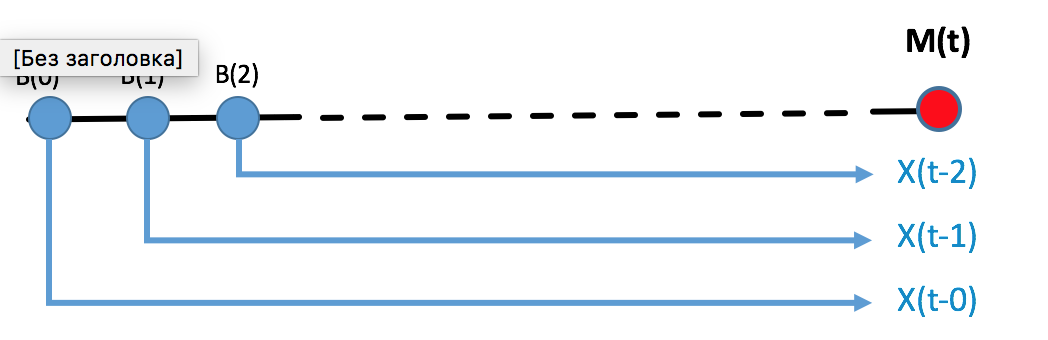
\includegraphics[height=5cm]{susceptibility}
  \caption{\small We break  up the force in time, and  mapping their effect using
    the susceptibility function, we can evaluate  the response of the system at a
    later time.}
\end{figure}

Two assumptions are made:
\begin{itemize}
\item  Linearity -  the effect  of  the different  forces $  X(t-t_i)B(t_i) $  is
  linearly summed up to find the resultant;
\item Causality implies that $ t_i < t  $, since the force cannot preceed its own
  effet.
\end{itemize}

\noindent to write the formula:

\begin{framed}\noindent
  \begin{equation}\label{eqn:response_2}
    M(t) = \int_{-\infty}^{t}X(t - \tau)B(\tau)d\tau.
  \end{equation}
\end{framed}

 \subsubsection{Sinusoidal Excitation}
 An excitation of the form:
 \begin{equation}
   B(t) = b\cos(\omega t) - ib\sin(\omega t) = be^{-i\omega t},
 \end{equation}

 \noindent  results  in  the  response  (where we  will  remmeber  manually  that
 $   X(t)   =   0  $   if   $   t<0   $,   so   the  limits   are   change   from
 Eq.~\eqref{eqn:response_2})

 \begin{equation}
   \begin{aligned}
     M(t) &= b\int_{-\infty}^{+\infty}X(t - \tau)e^{-i\omega \tau}d\tau\quad\text{chang of var}&\\
     & = be^{-i\omega t}\int_{-\infty}^{\infty}X(\tau)e^{ii\omega\tau}d\tau&\\
   \end{aligned}
 \end{equation}

 \noindent or more compactly
 \begin{framed}\noindent

   \begin{equation}\label{eqn:response_3}
     \begin{aligned}.M(t) &= be^{-i\omega t}\chi(\omega)\\ \chi(\omega) &= \int_{-\infty}^{\infty}X(\tau)e^{i\omega t}dt
     \end{aligned}
   \end{equation}

 \end{framed}

 \noindent  Because response  is  linear, if  we split  up  the frequency  domain
 susceptibility into real and imaginary components

  \begin{equation}
    \chi(\omega) = \chi'(\omega) + i\chi''(\omega),
  \end{equation}

  \noindent then the response to

  \begin{equation}\label{eqn:response_4}
    b\cos(\omega t) = \Re[be^{-i\omega t}]  =\Re[M(t)] = b\big[\red{\cos(\omega t)\chi'(\omega)} + \blue{\sin(\omega t)\chi''(\omega)}\big],
  \end{equation}

  \noindent with an \red{in-phase} and \blue{quadrature} components.

  Moreso, the unbound limits of Eq.~\eqref{eqn:response_3} mean that

  \begin{equation}
    \begin{aligned}
      \chi(\omega) & = \chi^{*}(-\omega)\\
      \chi'(\omega) = \chi'(-\omega)\\
      \chi''(\omega) = -\chi''(-\omega)\\
    \end{aligned}
  \end{equation}

  \noindent meaning that the real and imaginary parts of dynamical susceptibility
  are even and add respectively.

\begin{figure}[h]
  \centering 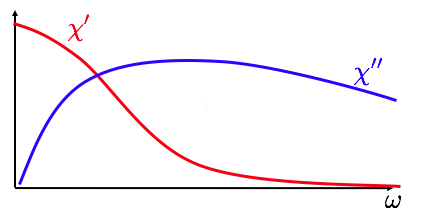
\includegraphics[height=5cm]{susceptibility_1}
\end{figure}

\newpage\subsubsection{Frequency representation}
\begin{framed}\noindent
  For this section we shall use definition of the FT:
  \[
    \begin{aligned}X(t) & = \frac{1}{2\pi}\int X(\omega)e^{-i\omega t}d\omega\\
      X(\omega) & = \int X(t)e^{i\omega t}dt
    \end{aligned}
  \]

\end{framed}
Eq.~\eqref{eqn:response_3}  describes   the  response  to  a   single  sinusoidal
exciation. Now  let us  consider that  the exciation is  a superposition  of such
sinusoids :

   \begin{equation}
     be^{-i\omega t} \iRa B(t) = \frac{1}{2\pi}\int_{-\infty}^{\infty}b(\omega)e^{-i\omega t}d\omega.
   \end{equation}

   Defining  $ m(\omega)e^{i\omega  t} $  as the  response to  one of  these sinusoids  (in
   Eq.~\eqref{eqn:response_3}) %(\red{we redefined the $ \pm $ in the exponentials for consistency})
   \begin{equation}\label{eqn:freq_1}
     \begin{aligned}
       {m(\omega)e^{-i\omega  t}   =  b(\omega)e^{-i\omega  t}\chi(\omega)}  \iratext{integrating   over  all
         $                                                                      \omega
         $ + normalising} &\\\\ \ M(t) = \frac{1}{2\pi}\int_{-\infty}^{\infty}m(\omega)e^{-i\omega t}d\omega &=
       \int_{-\infty}^{\infty}\chi(\omega)b(\omega)e^{-i\omega t}d\omega.
     \end{aligned}
   \end{equation}

   \noindent Fully this will all read

\begin{framed}\noindent
  Given a superposition of forces (expressed by $ b(\omega) $ in the frequency range)
  \begin{equation}\label{eqn:freq_2}
    B(t) = \frac{1}{2\pi}\int_{-\infty}^{\infty}b(\omega)e^{-i\omega t}d\omega,
  \end{equation}
  \noindent the response can be found by evaluating the response at frequency:
  \begin{equation}\label{eqn:freq_3}
    m(\omega) = \chi(\omega)b(\omega),
  \end{equation}
  \noindent and  `summing' them  up, which  is equivalent  to taking  the fourier
  transform
  \begin{equation}\label{eqn:freq_4}
    M(t) = \frac{1}{2\pi}\int_{-\infty}^{\infty}m(\omega)e^{-i\omega t}d\omega.
  \end{equation}
\end{framed}

\newpage \subsubsection{Step  excitation} A step  excitation is removed  from the
system at time $ t = 0 $

  \begin{equation}
    B(\tau) = b \text{ only for } \tau < 0.
  \end{equation}

  \noindent Evaluating Eq.~\eqref{eqn:response_2}

  \begin{framed}\noindent
    \begin{equation}\label{eqn:step_1}
      \begin{aligned}
        M_\text{step}(t)  \equiv& = b\int_{-\infty}^{0}X(t-\tau)d\tau\\
        & = b\red{\int_{t}^{\infty} X(\tau)d\tau} = b \red{\varPhi(t)} \\
        & \red{\Phi(t) \text{ - resonse of system to step function}}
        % & = b\varPhi(t) \qquad\qquad \varPhi(t) = \int_{t}^{\infty}
        % X(\tau)d\tau.
      \end{aligned}
    \end{equation}
  \end{framed}
  \subsubsection{Delta exciation}
  A delta excitation is only switched on at a certain time.
  \begin{equation}
    B(\tau) = b\delta(\tau)
  \end{equation}
  \noindent The selection mechanism of this function results in

  \begin{framed}\noindent
    \begin{equation}\label{eqn:delta}
      \begin{aligned}
        M_\delta(t) & = b\blue{X(t)} \equiv -b\frac{d}{dt}\red{\Phi(t)}\\
        & \blue{X(t) \text{ - resonse of system to delta
            function}} %\iratext{Eq.~\eqref{eqn:step_1}} M_\delta(t) = -b\frac{d}{dt}M_\text{step}(t) \red{= - \frac{d}{dt}}
      \end{aligned}
    \end{equation}
  \end{framed}

  \subsection{Summary}
  \begin{table}[h]
    \centering
    \caption{Refference table for responses\label{tab:responses}}
    \begin{tabular}{|c|c|c|}
      \hline\textbf{Excitation} & \textbf{Response} $ M(t) $ & \textbf{Special Response for b = 1}\\\hline
      $ b\cos(\omega \tau) $ & $ b\big[{\cos(\omega t)\chi'(\omega)} + {\sin(\omega t)\chi''(\omega)}\big] $ & \\
      $ b\theta_-(\tau) $ & $ b\int_{t}^{\infty}X(\tau)d\tau $ & $ \Phi(t) $\\
      $ b\delta(\tau) $ & $ bX(t) $ & $ X(t) $\\\hline
    \end{tabular}
  \end{table}

  \red{The delta function is minus the derivative of the step down function
    \[
      \delta(\tau) = -\frac{d}{dt}\theta_-(\tau).
    \]

    \textbf{Because our  system is  linear, any  relation between  the excitation
      will mirror itself in the response}

   \begin{equation}\label{eqn:delta_2}
     X(t) = -\frac{d}{dt}\Phi(t).
   \end{equation}}

\subsection{Energy}
If we  treat $ B(t)  $ as a  force and $ M  $ as a  displacement, then we  can in
general write that
\begin{equation}\label{eqn:energy_1}
  B = \frac{\partial\text{Energy}}{\partial M},
\end{equation}

\noindent and the power dissapation is then:

 \begin{equation}
   P = \iaverage{\ipartial{\text{Energy}}{t}} = \iaverage{B\frac{\partial M}{\partial t}}.
 \end{equation}

 \noindent Using an excitation of the from  for the response function $ M(t) $ we
 get

 \begin{equation}
   \begin{aligned}
     B & = b\cos(\omega t)\\
     M(t)    &    =    b\big[{\cos(\omega   t)\chi'(\omega)}    +    {\sin(\omega
       t)\chi''(\omega)}\big]
   \end{aligned}
   \iRa P = \omega b^2\big[-\chi'(\omega)\iaverage{\sin(2\omega t)/2} + \chi''(\omega)\iaverage{\cos^2(\omega t)}\big]
 \end{equation}

 \noindent  which  evalutes  to  ($   \iaverage{\sin(2\omega  t)/2}  =  0  $  and
 $ \iaverage{\cos^2(\omega t)} = 1/2 $)


 \begin{framed}\noindent
   \begin{equation}\label{eqn:energy_2}
     P = \frac{1}{2}b^2\omega\red{\chi''(\omega)}.
   \end{equation}
   \textbf{\red{Disspation that occurs  is proportional to imaginary  part of the
       susceptibility, $ \chi''(\omega) $.}}

\end{framed}
Using the definitions for working out the units of different quantities:
\begin{equation}
  \begin{aligned} \ira [\chi] = [M^2]/[\text{energy}].
    [M] &= [\chi][B] &&\text{from Eq.\eqref{eqn:response_3}}\\
    [B] & = [\text{energy}]/[M] &&\text{from Eq.~\eqref{eqn:energy_1}}
  \end{aligned}
\end{equation}
\begin{equation}\label{eqn:unit1}
  \begin{aligned} \ira [X] = [M^2]/[\text{energy}][\text{time}], [\Phi] = [M^2]/[\text{energy}].
    [M] &= [X][B][\text{time}] &&\text{from Eq.\eqref{eqn:response_2}}\\
    [B] & = [\text{energy}]/[M] &&\text{from Eq.~\eqref{eqn:energy_1}}
  \end{aligned}
\end{equation}


\begin{center}
  \begin{tabular}{|c|c|c|}
    \hline
    $ [\chi] $ & $ [X] $ & $ [\Phi] $\\
    $ [M^2]/[\text{energy}] $&$ [M^2]/[\text{energy}][\text{time}] $ & $ [M^2]/[\text{energy}] $\\\hline
  \end{tabular}
\end{center}

\newpage \subsection{Onsager's hypothesis}
% \textbf{Let  us derive and  expression for the frequency  domain susceptibility
%  $  \chi(\omega) $  from  the  observed  correlation  function of  the  systems
% response, be it voltage, current, etc}.
\begin{framed}\noindent
  \textbf{Let us make an assumption, (that  Onsager made), that after a step-like
    distrubrance, a  system, $ M_\text{step}(t)  $, regresses to  its equilibrium
    state in the same way as it would under a random fluctuation.
    % In other words, we can study the state of Xnon-equilibrium system
    % with an equilibrium approach. Which is understandable - at the
    % microscopic level, there is no concept of an equilibirum state
  }
\end{framed}
\begin{equation}
  \left\lbrace\begin{aligned}
      M_\text{step}(t) & = \beta\iaverage{M(0)M(t)} && \text{according to Onsager, regression same as equilibium one}\\
      M_\text{step}(t) & = \beta\Phi(t) && \text{when we deal with step excitation as in Table.~\ref{tab:responses}}\\
      X(t) & = -\frac{d}{dt}\Phi(t) && \text{definition of dynamical susceptibility}
    \end{aligned}\right.,
\end{equation}

\noindent  where $  \beta $  is a  constant, which  for classical  mechanics, and
quantum treatment at high temperatures, reduces to $ \frac{1}{kT} $.

The Fourier Transform (only need to do it after the reponse at t=0 has occured)

\begin{equation}\label{eqn:susceptibility_from_response_0}
  \begin{aligned}
    \chi(\omega) & = \int X(t)e^{i\omega t} dt\\
    & = -\frac{1}{kT}\int_0^\infty\iaverage{M(0)\dot{M}(t)}e^{i\omega t}dt\\
    & = \left.\iaverage{M(0)M(t)}e^{i\omega t} \right|_0^\infty - - \frac{1}{kT}i\omega\int_{0}^\infty\iaverage{M(0)M(t)}e^{i\omega t}dt\\
    & = \chi_0 + \frac{i\omega}{kT}\int_{0}^\infty\iaverage{M(0)M(t)}e^{i\omega t}dt\\
  \end{aligned}
  % -\frac{1}{kT}
\end{equation}

\begin{framed}\noindent
  For  a step  like disturbance,  the  susceptibility function  in the  frequency
  domain can be evaluated using
  \begin{equation}\label{eqn:susceptibility_from_response}
    \chi(\omega) = \chi_0 + \frac{i\omega}{kT}\int_{0}^\infty\iaverage{M(0)M(t)}e^{i\omega t}dt
  \end{equation}

\end{framed}

\noindent Converting to the usage of $ \Phi(t) $ instead of $ M_\text{step}(t) $,
we  need  to add  a  normalisation  factor  $ \beta  $  to  keep the  units  from
Eq.~\eqref{eqn:unit1}

\begin{equation}\label{key}
  \begin{aligned} \ira X(t) = -\frac{1}{kT}\iaverage{M(0)\dot{M}(t)}
    \Phi(t) &= \beta\iaverage{M(0)M(t)}\\
    \Phi(t) &= -\frac{dX(t)}{dt}
  \end{aligned}
  % \chi(\omega) = \int_{-\infty}^{+\infty}X(\tau)e^{i\omega t}dt =
\end{equation}

\noindent where, without going into too much depth, $ \beta = \frac{1}{kT} $ from
equipartition  (derived  in  the  last  chapter  of  the  book).   The  dynamical
susceptibility, evaluated for after the excitation,

\begin{framed}\noindent
  \begin{equation}\label{eqn:onsager_1}
    \chi(\omega) =
    -\frac{1}{kT}\int_{0}^{\infty}\iaverage{M(0)\dot{M}(t)} %\xi_0+\frac{i\omega}{kT}\int_{0}^{\infty}\iaverage{M(0){M}(t)}e^{i\omega t}dt
  \end{equation}
  \red{So if we  know the autocorrelation function of a  systems response, we can
    evaluate the dynamic susceptibility,}

\end{framed}

 \subsection{Charge and current}
 Consider the  step to  be voltage, $  B \ilra  V $, and  the response  a charge,
 $  M   \ilra  Q  $.    \textbf{\red{We  can   monitor  the  charge   Q}}.   Like
 Eq.\eqref{eqn:freq_2},\eqref{eqn:freq_3}:

 \begin{equation}\label{key}
   \begin{aligned}
     Q(t) & = \int X(t-\tau)V(t)d\tau\\
     q(\omega) & = \chi(\omega)v(\omega),
   \end{aligned}
 \end{equation}

 \noindent \red{$ \chi(\omega)  $ being the frequency  dependent capacitance}. As
 we saw in Eq~\eqref{eqn:energy_2}, its  imaginary part will lead to dissapation,
 $     P     =\iaverage{B\frac{dM}{dt}}     =     \iaverage{V\frac{dQ}{dt}     }=
 \frac{1}{2}b^2\omega\red{\chi''(\omega)}. $

 Above in  Eq.~\eqref{eqn:susceptibility_from_response_0} we  have seen  how this
 capacitance  susceptibility,  $  \chi(\omega)  $, can  be  calculated  from  the
 response, $ Q(t) $

 \begin{equation}\label{key}
   \begin{aligned}
     \chi(\omega) & = -\frac{1}{kT}\int_{0}^\infty\iaverage{Q(0)\dot{Q}(t)}e^{i\omega t}dt = -\frac{1}{kT}\int_{0}^\infty\iaverage{Q(0)\green{I(t)}}\green{e^{i\omega t}}dt \\
     & \text{not trivial, but you don't need to do it}\\
     & = \frac{i\omega}{kT}\int_{0}^{\infty}\iaverage{I(0)I(t)}e^{i\omega t}dt
     % & = \left.\iaverage{Q(0)\green{Q(t)}}\green{e^{i\omega
     %   t}\frac{1}{i\omega}}\right|_0^\infty +
     % \frac{1}{kT\green{i\omega}}\int_{0}^{\infty} \\
     % & = \left.\iaverage{M(0)M(t)}e^{i\omega t} \right|_0^\infty - -
     % \frac{1}{kT}i\omega\int_{0}^\infty\iaverage{M(0)M(t)}e^{i\omega
     % t}dt\\
   \end{aligned}
   % \frac{1}{Z(\omega)} = i\omega c(\omega) = i\omega \chi(\omega)
   % \frac{-i\omega}{kT}\int_{0}^{\infty}\iaverage{Q(0)\dot{Q}(t)}e^{i\omega
   % t}dt.
 \end{equation}

 \begin{framed}\noindent
   \noindent Or in terms of the  Impedance $ Z = \frac{1}{i\omega \chi(\omega)} $
   (equation for capactitive impedance)

  \begin{equation}\label{key}
    \frac{1}{Z(\omega)} = \frac{1}{kT}\int_{0}^{\infty}\iaverage{I(0)I(t)}e^{i\omega t}dt.
  \end{equation}
  The  impedance  of  an  object  is  related  to  the  area  under  the  current
  autocorrelation graph.

  And           this           is          different           from           the
  $ \frac{1}{R}=\frac{1}{2kT}\int\iaverage{I(0)I(t)}dt $  expression form before,
  because now  we are getting the  impedance at a particular  frequency, not just
  the  general  one.   (In fact  its  just  the  above  intergrated for  all  the
  frequencies).

\end{framed}

\newpage
